\documentclass[8pt]{beamer}

\setbeamertemplate{background canvas}[vertical shading][bottom=cyan!10,top=blue!10]

\usetheme{Warsaw}
\usefonttheme[onlysmall]{structurebold}

% pour le fichiers .pdf
\usepackage{graphicx}
\usepackage{color}
% pour les fichiers .png
% \usepackage{pgf,pgfarrows}
% \usepackage{pgf,pgfarrows}
\usepackage{amsmath,amssymb}
\usepackage[latin1]{inputenc}
\usepackage[T1]{fontenc}
\usepackage[french]{babel}
\usepackage{textcomp}
\usepackage{Math_Notations}
\usepackage{multitoc}
\usepackage{mdwtab}
\setbeamercovered{dynamic}
\DeclareMathOperator*{\argmin}{argmin}

\title[OpenTURNS Developer training]{OpenTURNS Developer training: first steps with OpenTURNS}
\author[R. Lebrun, copyright EADS 2011.]
{
  Trainer : R�gis LEBRUN, EADS/IW/SE/AM
  regis.lebrun@eads.net
}



\date[March 22-25th 2011]
{
  Developers training \\

  \begin{center}
    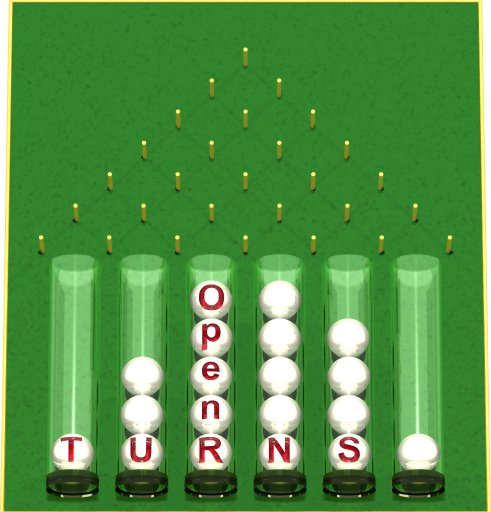
\includegraphics[height=2cm]{logoOT.jpg}
  \end{center}
}

\subject{OpenTURNS Developers Training}

% \part<presentation>{Corps de presentation}


\begin{document}

\frame{\titlepage}

% necessaire pour la table des matieres
\part{Main part}

% table des matieres
\begin{frame}
  \frametitle{First steps with OpenTURNS}
  \tableofcontents[part=1]
\end{frame}
%%%%%%%%%%%%%%%%%%%%%%%%%%%%%%%%%
% Navigation in the source code %
%%%%%%%%%%%%%%%%%%%%%%%%%%%%%%%%%
%%%%%%%%%%%%%%%%%% 
% Global picture %
%%%%%%%%%%%%%%%%%% 
\begin{frame}
  \frametitle{Navigation in the source code}
  \begin{block}{The Uniform distribution}
    \begin{itemize}
      \item Locate the class within the library source code;
      \item Follow its inheritance graph in order to explore the Bridge pattern;
      \item Locate the associated regression test;
      \item Execute the test;
      \item Locate its SWIG interface file and its associated Python module;
      \item Execute the associated python test.
    \end{itemize}
  \end{block}
\end{frame}
\end{document}

